\documentclass[a4paper,11pt]{report}

%%%% PREAMBLE
\usepackage{pdfpages}
\usepackage{scrextend}
\setlength\parindent{12pt}
\usepackage{graphicx}
\usepackage{subfig}
\usepackage{float}
\usepackage{relsize}
\usepackage{amsmath}
\usepackage{amssymb}
\usepackage{textcomp}
\usepackage{hyperref}
\usepackage{lscape}
\usepackage{longtable}
\usepackage{gensymb}
\hypersetup{
    colorlinks=true,
    linkcolor=blue,
    filecolor=magenta,      
    urlcolor=cyan,
}

%\usepackage[margin=1.0in]{geometry}

%%%%  Add some length to the page, as margins always seem too big.  
\addtolength{\topmargin}{-1.5in}
\addtolength{\textheight}{2in}

\begin{document}

%%%%  Number the initial front matter with roman numerals
\pagenumbering{roman}


%%%%  TITLE PAGE
%%  Here are the elements that make up the title page of the document.  

\thispagestyle{empty}  %%  Make the title page have no number.  

%%%%  INSERT TITLE AND NAME HERE!!
\title{\LARGE
Creating a Geospatial Macro Level Feature Database}

\author{Jason Brewer
\\    \\    \\
Specification and Proposed Design
\\    \\
Submitted to 
\\    \\    \\ 
The University of Liverpool
\\    \\
\\    \\
in partial fulfilment of the requirements
\\
for the degree of 
\\     \\
MASTER OF SCIENCE
\\     \\    \\    \\
}


%%  Fill in a date here if you want, or comment out the line below and
%%  the current date will be automatically inserted for you.  
\date{\today}


\maketitle

\newpage

%%%%  TABLE OF CONTENTS  
%%%%      Usually the following command will give you the formatting you want.  

\tableofcontents

%% declaration of whatever is not needed in this document

%%%%  LIST OF FIGURES
%%%%      Comment out this line if you have no figures in your document.  
%\listoffigures


%%%%  LIST OF TABLES  
%%%%      Comment out this next line if you have no tables in your document.  
%\listoftables


\newpage

%%%%  Turn page numbering back to arabic.  This also resets the numbering
%%%%  to begin again at page 1.  

\pagenumbering{arabic}

%%%%  INTRODUCTION

\chapter{Summary of Proposal}\label{chap:summ}

\section{Overview} \label{overview}

Blind or visually impaired (BoVI) individuals face many day to day issues regarding the ability to navigate the outdoor world with confidence. As highlighted by Quinonoes et al. \cite{quinones_supporting_2011}, a given hardware and software system for BoVI users must address navigation focussing on recovery from mistakes on a given route, losing one's way, unfamiliar routes and changes to a route which the system must react to efficiently and robustly. 

By understanding the needs of the BoVI user, it becomes apparent that a system must be able to identify meaningful waypoints on a given outdoor route whilst at the same time not supplying an overwhelming amount of information. In effect, the system must act like a background process with an occasional element of interactivity: gathering useful information about the world as it would be perceived by a sighted person and, when required, relaying relevant information back to the BoVI user when required.

A broad overview of a proposed system is shown below in the form of a mind-map in figure \ref{fig:mindmap}. A publicly available (and more readable) version can be found at \url{http://bit.ly/2sgygt6}. This can be thought of as a physical representation of preliminary brainstorming. It was devised in the pre-planning phase of the development. This document is a record of the planning phase proper.

% figure out a way to make this a single landscape page so it can be read somewhat easily by the final reviewer
% play about with [h] and [H] (nope). 

\begin{figure}
	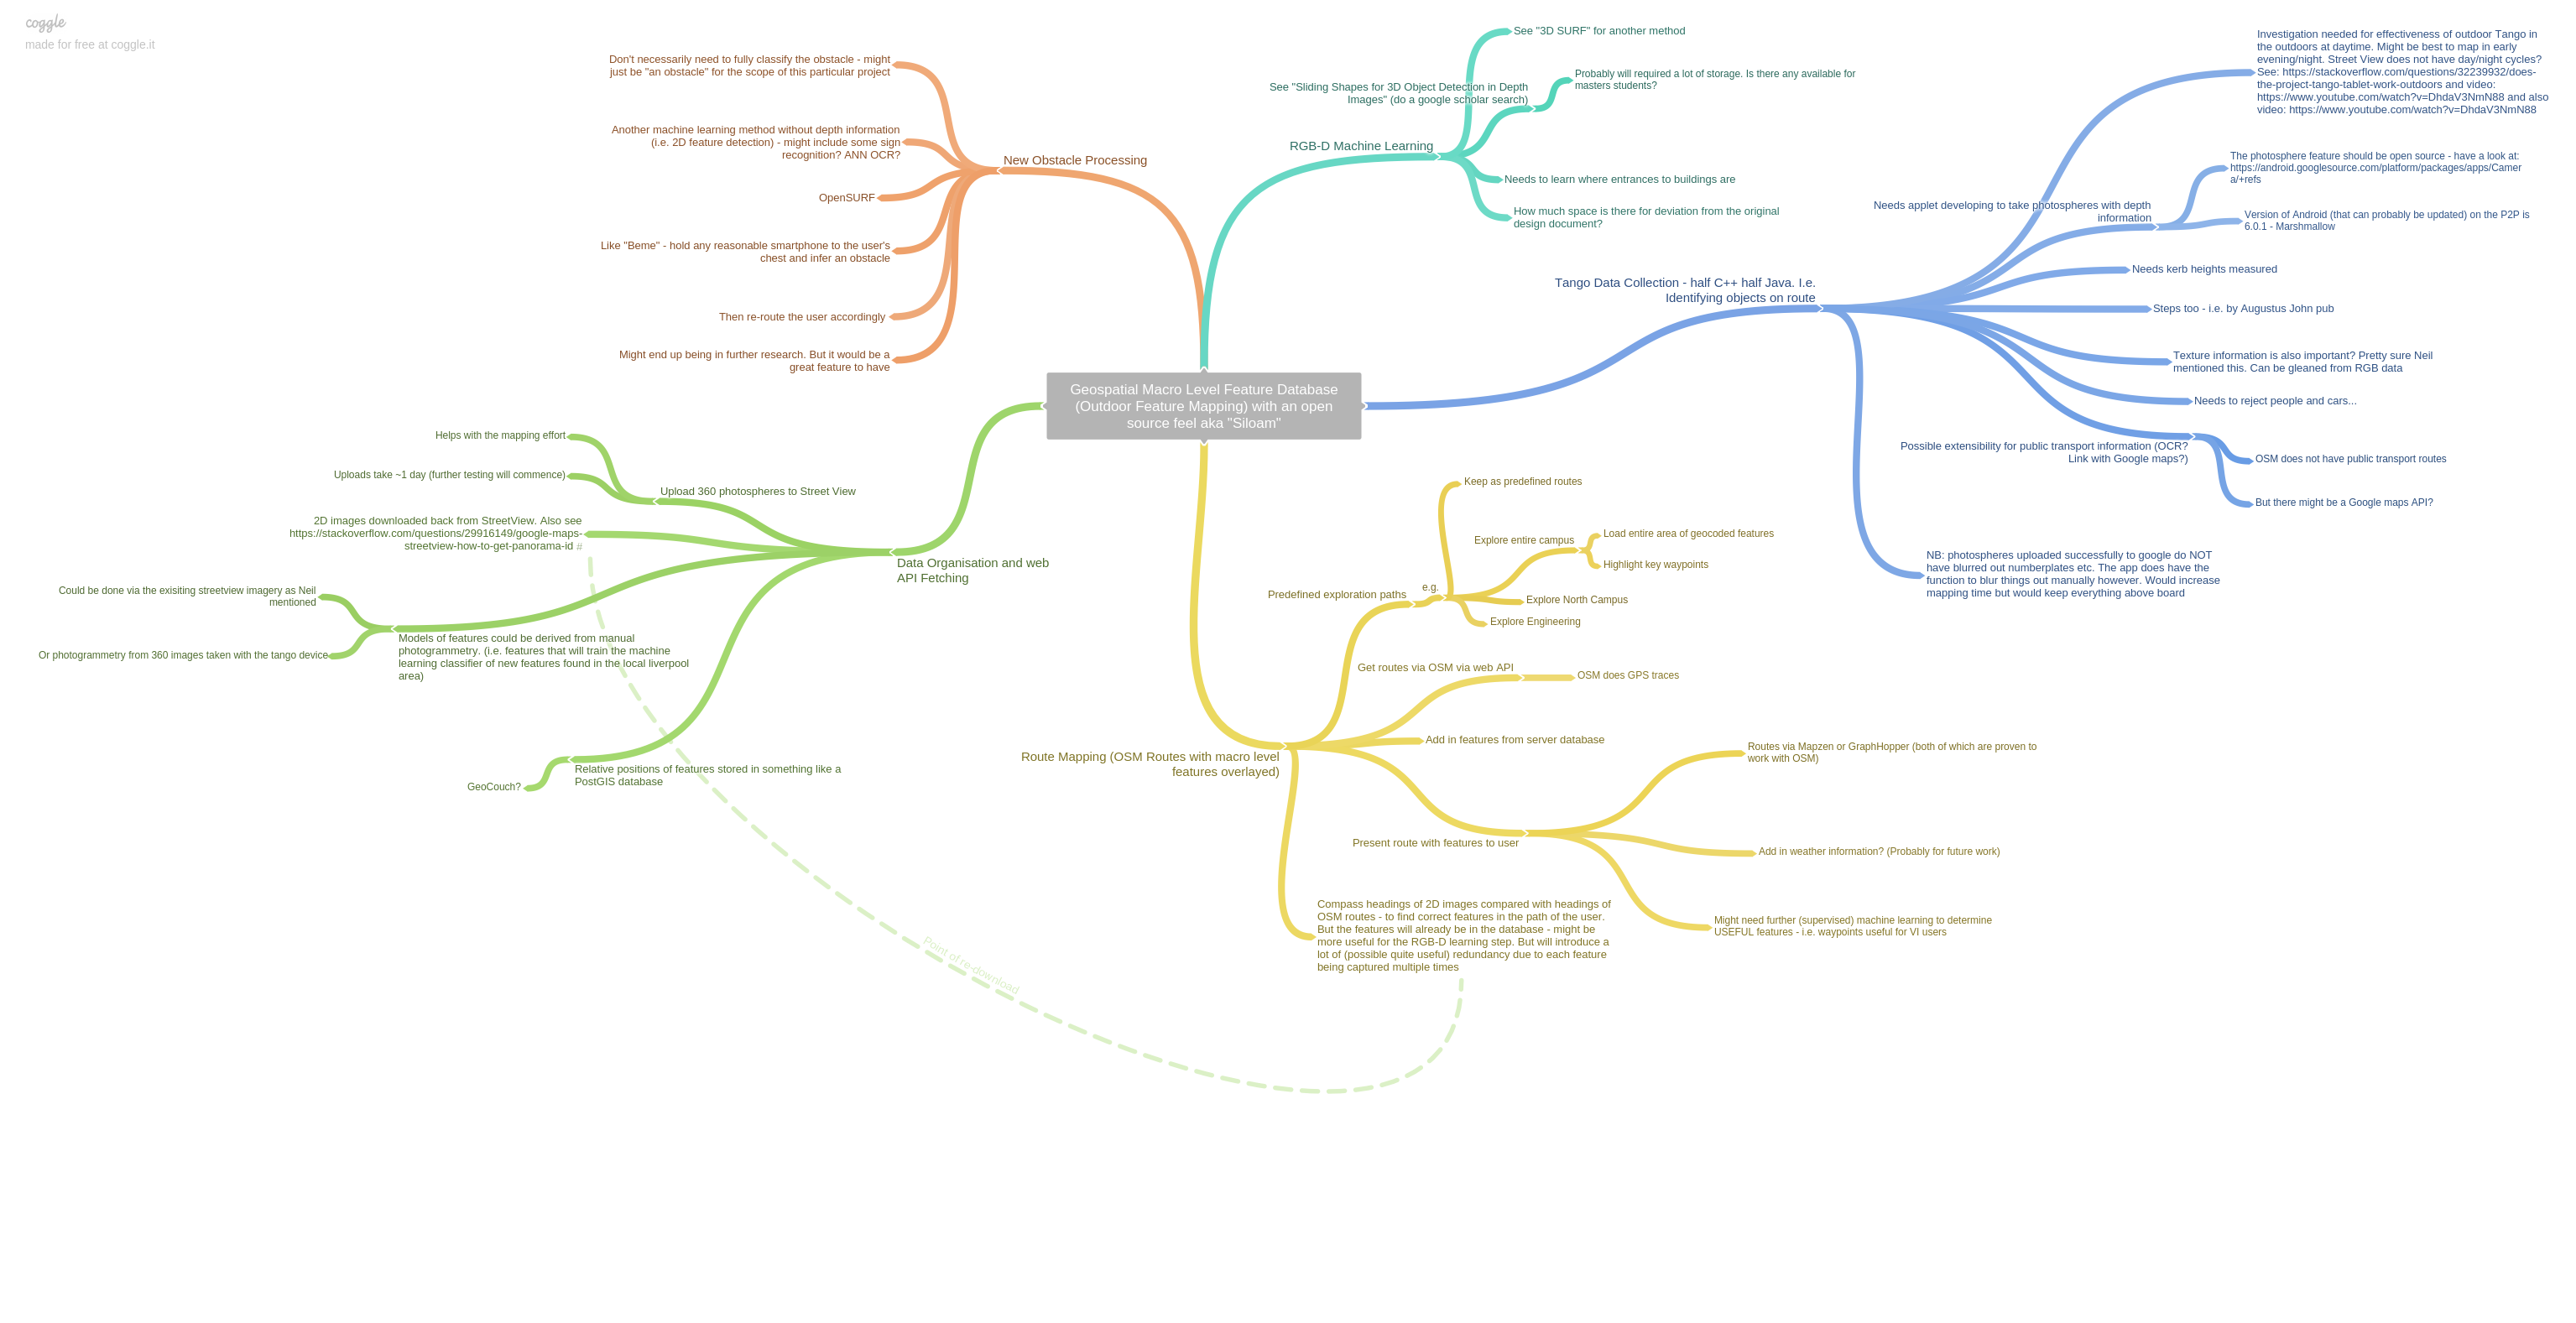
\includegraphics[scale=0.246, angle=90]{mindmap}
	\caption{Project Overview}
	\label{fig:mindmap}
\end{figure}

Figure \ref{fig:mindmap} shows five distinct subsystems that are represented by the main arms of the map, in the order of development and execution flow:

\begin{itemize}
	\item \textbf{data collection}
	\item \textit{RGB-D machine learning}
	\item \textbf{data organisation}
	\item route mapping
	\item new obstacle processing
\end{itemize}

Development will be carried out in conjunction with another University of Liverpool student who will be covering the items above not in bold face in a separate report. They will be covered only briefly to put the topics in bold face \textbf{(that will be covered in this document)} in context. Topics in italics are to be developed jointly because of their scale.

\section{Non-technical Summary}

To define the experimental scope a prototype system, a geographical area must be defined that is small enough to be considered viable for evaluation. The area chosen is the University of Liverpool (UoL) campus as it is known to have poor levels of 3D mapping data. The campus also has enough physical area for "exploration" type behaviour whilst at the same time having a number of routes of varying length that can be used for verification and evaluation purposes. 

In simple terms, combined parts of the prototype will effectively map out the area in question, automatically identify all street level features, (for example: bus stops, lamp posts, kerb heights, doorways, pedestrian crossings, steps etc) and save their positions in space. Referring to the five distinct subsystems in figure \ref{fig:mindmap},  a Google project Tango \cite{noauthor_tango_nodate} (referred to as ``Tango'' throughout this document) enabled device, the Lenovo Phab 2 Pro, will be used to gather 3D models of each of these macro features with their position on the campus, which will then be stored on a laptop. This is the ``data collection'' subsystem. Another application will then work out what these features are, after which they will be stored on a publicly accessible database. These are the ``RGB-D machine learning'' and ``data organisation'' subsystems respectively. The Phab 2 Pro is the only Tango enabled device that is readily available in Europe and, contrasting to the Tango Yellowstone development tablet, is more available to the wider world, particularly important as 90\% of the world's BoVI people are in the developing world \cite{jafri_gps-based_2014}. The design and testing of these three subsystems will form a well defined standard whereby any given geographical location can be described by its macro level features. 

During use of a hypothetical mobile application, route mapping will be used to define a single destination point from the device's current geographical position or the centre of an exploration area. This subsystem will gather information about the location of useful waypoints along the route or in the general area as well as contact the pre-populated database as described above for street level features. Theses features and waypoints will be used to guide the BoVI in their navigation of previously uncharted spaces via a text-to-speech interface. Google's ``text-to-speech'' and Apple's ``VoiceOver'' could be used for this purpose. 

The final subsystem is used to identify new obstacles or hazards that are not defined in the collection of features known to the database, for example routine pavement maintenance work or the relocation of a bus stop. To accomplish this, the user will hold their smartphone up to their chest and a geocoded picture will be taken. From this picture, a profile of the obstacle will be ascertained and the database will be updated. The user will be re-routed accordingly. At such time when the obstruction is cleared, the user will take another picture of the view of the cleared path and the database will again be updated so that re-routing is not performed unnecessarily in the future.             

\section{Technical Summary}\label{sec:techSummary}

At the pre-project phase, an idea for the macro level features to be gathered from existing street imagery was considered. There are two problems with this approach. First, since much of the UoL campus is pedestrianised, street imagery from a publicly available source like Google Street View is not available. This constraint requires extra mapping of the area to be done anyway. So called ``photo spheres'' (360\degree{} photographs that are interactively viewable with a set of geometrical transforms) are the backbone of Street View and can be captured with any reasonable smartphone. Secondly, on review of StreetView data, there are inconsistencies in the date a given geographic area was captured. For example, photo spheres for a given street might have a copyright date of 2016 but a neighbouring street may have a copyright (and therefore publishing) date of 2008. Discrepancies of this sort will be solved in time, after all Google's capture mechanisms cannot be online 24 hours a day, but trying to use data at this level of inaccuracy for a project of this type would be inappropriate. 

Therefore, it is suitable for a new data collection effort using a the previously mentioned Tango device, the Phab 2 Pro, to capture photo spheres with image (RGB) as well as depth data (D), together forming RGB-D data, simultaneously. The Phab 2 Pro has an array of sensors, including a time of flight infra-red emitter receiver pair and a 100fps global shutter fish eye camera, to perform simultaneous localisation and mapping (SLAM \cite{choset_topological_2001}).  A mobile application using the Tango C/C++ API \cite{noauthor_getting_nodate} allows the developer to store both 3D mesh and texture information from RGB-D photo spheres. An geocoded array of these models can be used to build a collection of macro level features on the mapping route. Each RGB-D photosphere is then extracted from the mobile device onto a Macintosh (OSX 10.11.6) development machine. Macro level feature models are then separated from an estimation of the floor area using the RANSAC \cite{fischler_random_1981} algorithm and, taking inspiration from Fehr et al. \cite{fehr_covariance_2016}, categorised using a support vector machine (SVM) with a radial basis
function (RBF) kernel. This design decision is explored in section \ref{techResearch}.
Once feature categories are learned, their type and physical dimensions are encoded in JavaScript Object Notation (JSON) format and transferred to an Apache CouchDB \cite{noauthor_couchdb:_2017} database with the GeoCouch \cite{noauthor_geocouch:_2017} extension to allow spatial indexing and queries. This data can then be accessed via a representational state transfer (RESTful) API for route mapping and exploration area purposes. 

Any system that requires the new collection of geographical data will face a similar problems than that of Street View: it is non-trivial to update mapping information in real time. This is why a community driven, new obstacle detection is proposed. The user will hold their phone up to their chest, hence covering the proximity sensor present on the fact of the vast majority of modern smartphones. A photograph of the view in front of the user will then be taken. A trained machine learning algorithm would then detect the type of obstacle, and send this information along with GPS and magnetometer data from the smartphone to the database. This new information would be made available to other users on the network. This, however, is complex implementation.. A simpler method could rely on  is that obstacles not found in the database could be marked by a "partial" or "total" flag by the user, resulting different re-routing options. Implementation of this feature is however outside the scope of this document.

\section{Research and Analysis} 

\subsection{Current System Research}

Preliminary research of current systems for BoVI users shows that while they address many issues in a novel fashion, they do so separately and therefore do not represent an end to end navigation solution. Furthermore, solutions are frequently based on hardware that may no longer be available, are not currently be developed actively or are prohibitively expensive.

The work of Jafri and Khan \cite{jafri_obstacle_2016} seems to be mirrored in Cydalion \cite{noauthor_cydalion._nodate}, an mobile application for Tango enabled devices that detects objects in the user's path and suggests effective avoidance in real time. Whilst focused on indoor environments, this technology could extended to be used outdoors. Jafri and Ali \cite{jafri_gps-based_2014} describe a system to record frequently used routes of BoVI users but fall short of implementing a working prototype. Entirely focussed on the outdoors with a wealth of information gathered from Google, Ariadne GPS \cite{author_ariadne_nodate} gives feedback via Apple VoiceOver on where they are located in the form of street numbers. It also gives the user a compass heading and estimated distance when in close proximity to waypoints that can be saved as favourites. Ariadne however offers what could be an overwhelming amount of information to the user at a distracting rate. Research from Microsoft allied with technology from Pivothead produced the Seeing AI project \cite{noauthor_seeing_nodate} which uses computer vision techniques to describe what is happening in the field of view of a glasses mounted, forward facing camera down to the detail of the age, sex and expressions of faces detected in the scene. Whilst promising, unfortunately this technology is currently in the private domain of Microsoft. 

\subsection{Technical Research} \label{techResearch}

Aside from Seeing AI, current systems use publicly available data in an attempt to help BoVI users build a mental map of their surroundings. Since the system proposed in this document will make use of machine learning techniques to identify macro level features, an in depth study of state of the art learning techniques is required.

Further work from Jafri \cite{jafri_gpu-accelerated_2017} describes the use of the internal graphics processing unit (GPU) of the Tango Yellowstone development tablet to perform object and face detection in real time. This and the previous work of Jafri and Khan \cite{jafri_obstacle_2016} would be useful, but much like the NAVI \cite{zollner_navi_2011} system involves unwieldy harnesses and other apparatus to achieve its goals. Systems like these have motivated the use of the five separate phases outlined in section \ref{overview} which, considering the battery life of current Tango devices (reportedly less than one hour during operation of the Tango sensor array), split the data collection and processing and only required the BoVI user's smartphone to connect to the server where macro level feature information for a given route or exploration radius is stored. Once information is downloaded from the server, it can be stored locally on any smartphone with accurate GPS/assisted GPS.

In the years following the public release of the Microsoft Kinect and its associated software development kits, a wealth of research was carried out in the domain of RGB-D image classification verified against a number of annotated datasets \cite{silberman_indoor_2012, song_sun_2015, lai_large-scale_2011, browatzki_going_2011}. Some recent works focus on the use of sliding windows to fit bounding boxes around objects in a 3D scene using an ensemble of exemplar SVMs \cite{song_sliding_2014} and deep 3D convolutional neural networks (DCNNs) \cite{song_deep_2016}. Shao et al. \cite{shao_performance_2017} present a comprehensive study of various types of neural networks for feature learning of RGB-D datasets, concluding that convolutional neural networks (CNNs) are superior to other methods including deep belief networks (DBNs), stacked denoising autoencoders (SDAEs) and long short term memory neural networks (LSTMs). Particularly relevant to this project (for which there is close to no annotated training data) is the weakly supervised CNN proposed by Sun et al. \cite{sun_weakly-supervised_2017}. Describing two separate DCNNs trained on ImageNet \cite{deng_imagenet:_2009} and ModelNet \cite{noauthor_princeton_nodate} respectively. The system combines the outputs of these networks and passes them into a Gaussian process classification (GPC) module. While DNN or exemplar SVM approaches may seem like panace\ae, it is important to note that training of such networks takes many hours or even days on powerful graphics processing units (GPUs). The use of such technology, whilst producing satisfactory precision recall (PR) curves, is expensive and does not promote accessible further research at this level of education.

Fehr et al. \cite{fehr_covariance_2016} propose an SVM with an RBF kernel using covariance based descriptors to reduce the dimensionality of a given feature descriptor of an RGB-D instance to 190, contrasting to dimensionalities in a range up to 188300 as presented by Bo et al. \cite{bo_unsupervised_2013}. Such a compact descriptor dramatically increases the speed of SVM training and testing by several orders of magnitude in a project such as this without too much of a performance penalty and will serve well as a proof of concept for the system. It has also been empirically shown to be scale invariant. Fehr at al. make use of the RANSAC \cite{fischler_random_1981} algorithm to estimate the floor region of the RGB-D images in their experiments but another method presented by Golovinskiy and Funkhouser \cite{golovinskiy_min-cut_2009} uses a min-cut approach.


For training, testing and normal operation of the various machine learning systems outlined these works, it is common to find that inputs are in the form of RGB-D data of various objects rendered from many different view points. Song and Xiao \cite{song_sliding_2014} gathered a collection of 3D models from Trimble Warehouse \cite{trimble_inc._3d_nodate} for common indoor objects, rendered them from many different angles and generated an array of depth maps. Fehr et al. used a similar method to train their SVM \cite{fehr_covariance_2016}.        

%%%%  DESIGN

\chapter{Design}\label{chap:design}

\section{Methodology}

Taking inspiration from the dynamic systems development method (DSDM) \cite{bittner2002use}, the design of the various parts of the system are prioritised using the \textbf{M}o\textbf{SC}o\textbf{W} \cite{brennan2009guide} principle, that is what the system: 

\begin{itemize}
	\item \textbf{M}ust have
	\item \textbf{S}hould have
	\item \textbf{C}ould have
	\item \textbf{W}on't have this time
\end{itemize}

With these constraints, we can reason that this first iteration of this design \textbf{M}ust have: data collection, organisation and machine learning as these constitute the idea of making a standard for data collection. It \textbf{S}hould have: an exploration radius (or at least bounding box) search function for returning macro level features in an unfamiliar location to the user. It \textbf{C}ould have: macro level features returned in the geometry for a specific route. It \textbf{W}on't have this time: above 90\% machine learning accuracy probably due to lack of GPU accelerated deep learning, full audio feedback of surrounding features via mobile app, machine learning of new obstacles from RGB images without depth information.

Since this project is intended to produce a prototype, only the prototyping and testing aspects of the DSDM are covered here. In a sense interaction with supervisors, especially since development is taking place under the guidance of a representative from the Science and Technology Facilities Council (STFC), can loosely be seen as miniature workshopping events in themselves.  

\section{System Design} \label{sysDesign}

\subsection{Naming Conventions}

For the remainder of this document the proposed system as a whole will be referred to as ``Siloam'', named after the Pool of Siloam, where Jesus allowed a BoVI man to see. In each of the figures in this chapter, each subsystem is also referred to by a different name. In the order they appeared in section \ref{overview}, ``Data Collection'' is now referred to as ``SiloamSee''. ``RGB-D machine learning'' becomes ``SiloamLearn''. ``Data organisation'' becomes ``SiloamSilo'' and finally ``route mapping'' becomes ``SiloamRoute''.

\subsection{Overview}

Figure \ref{fig:SOverview} shows an overview of the whole system with general notes, including some parts of the design that have not yet been finalised in conjunction with my colleague and developer of SiloamRoute.

\begin{figure}[h]
\centering
	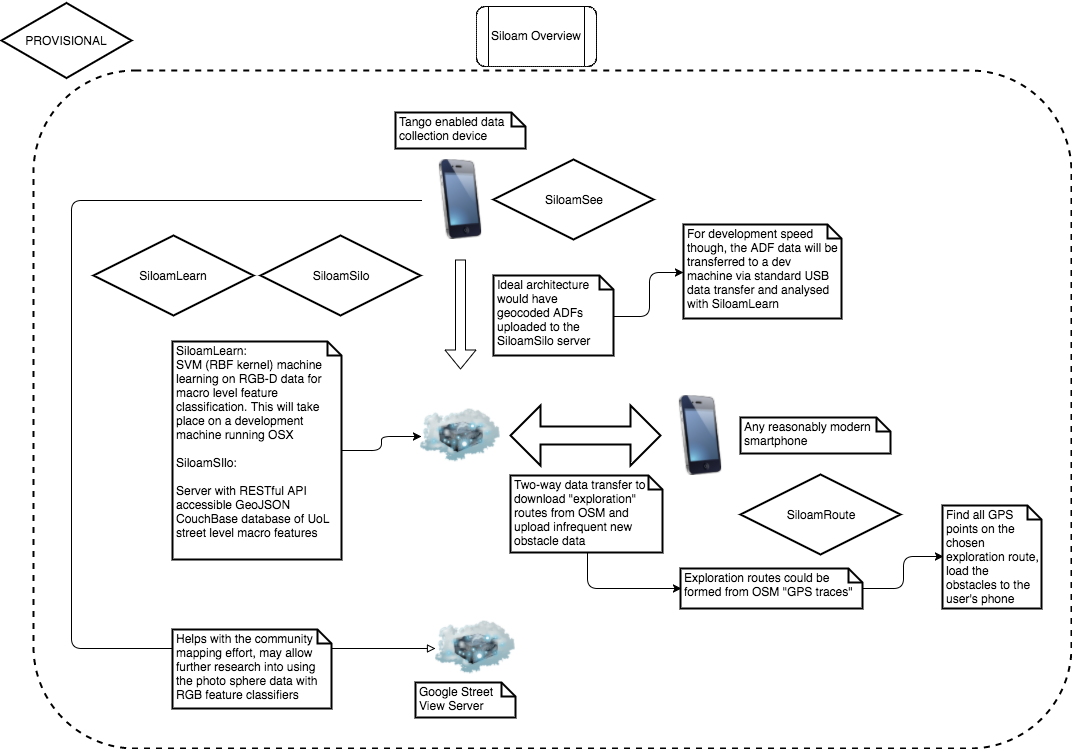
\includegraphics[scale=0.39]{SiloamOverview}
	\caption{SiloamOverview}
	\label{fig:SOverview}
\end{figure}

\subsection{SiloamSee}\label{secSSee}

Literature documenting the performance of various machine learning algorithms for the classification of indoor objects is numerous, principally because large RGB-D datasets are available for this purpose as mentioned in section \ref{techResearch}. Added to this, in the case of laboratory experiments involving live data capture, lighting conditions are easily controlled and changes in weather conditions are not a factor. Ren et al. \cite{ren_rgb-d_2012} highlight the opposite and pose the case that indoor scenes are poorly lit. While this is true, outdoor lighting conditions during extended data capture sessions (like ones required using SiloamSee) can change in a split second when direct sunlight illuminates objects after cloud occlusion which presents a challenge for comparing models of similar 3D meshes captured outdoors with a Tango device. 

Figure \ref{fig:SSee} shows an overview of the design of the SiloamSee component of the design, with notes. This will be developed as a small application for Android in Java with elements of the Tango C/C++ API \cite{noauthor_getting_nodate} and the open source Android camera application available for Android version 6.0.1 which runs on the Phab 2 Pro. The user interface (UI) component will principally be inherited from the Android camera app, but will add in elements of the Tango API to capture depth data whilst also capturing images that can be stitched together to create an equirectangular Plate Carr�e projection - that is a photo sphere. The RGBDPhotoSphere class will be responsible for capturing, rendering each geocoded photo sphere and finally uploading to Google servers via the Street View publish API \cite{noauthor_street_nodate}. During the capture of the photo sphere, the Tango specific sensors will build up an area description file (ADF) which will store a 3D mesh of the immediate surroundings within a 3 metre super-hemispherical area with a minimum located on the current plane of the ground, since depth information cannot be captured towards the sky unless in an enclosed space.

Another challenge with outdoor data collection with the Phab 2 Pro is the influence of direct sunlight. The time of flight (ToF) infra-red (IR) sensor will be heavily influenced by IR radiation from the sun reflected off surfaces. For this reason, data collection will take have to take place in early evening or on overcast days. Reflective surfaces like glass and also very dark coloured surfaces also pose a problem because IR light from the ToF sensor are reflected in unexpected ways or are absorbed. This in turn leads to inaccurate texture data. 

The work of Labb\`e  and Michaud \cite{labbe_memory_2011,labbe_online_2014}, available in the open source project RTAB-Map \cite{noauthor_rtabmap:_2017}, will be a useful source of inspiration for generating a collection of 3D meshes. Meshes will be captured along predefined routes throughout the UoL campus to be processed and used as training data by the SiloamLearn component. Also included in the data capture process will be the measuring of kerb heights, which, if applicable to the current capture area, the application will prompt the user to measure every 2 metres to ensure variations are recorded. 

\begin{figure}[h]
\centering
	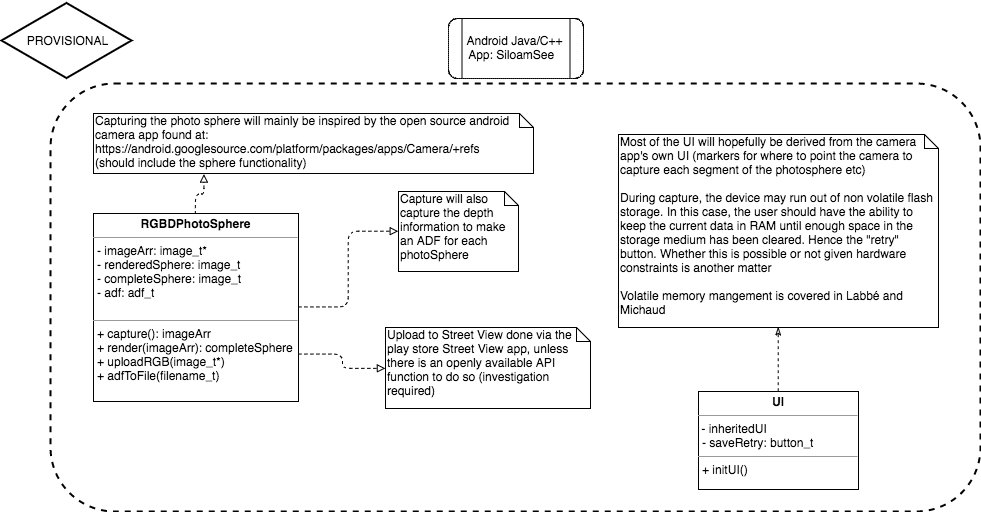
\includegraphics[scale=0.39]{SiloamSee}
	\caption{SiloamSee: Data Collection}
	\label{fig:SSee}
\end{figure}

\subsection{SiloamLearn}\label{secSLearn}

SiloamLearn has three tasks: extract the macro level features from each of the 3D meshes from SiloamSee, train an SVM with RBF kernel as detailed in Fehr et al. \cite{fehr_covariance_2016} and finally forge a connection with SiloamSilo to transfer the geocoded macro level features. The SVM used by Fehr et al. makes use of LIBSVM, for which both C++ source and implementation are available \cite{chang_libsvm:_2011}. Figure \ref{fig:SLearn} shows an overview of the subsystem, with notes. 

\begin{figure}[h]
\centering
	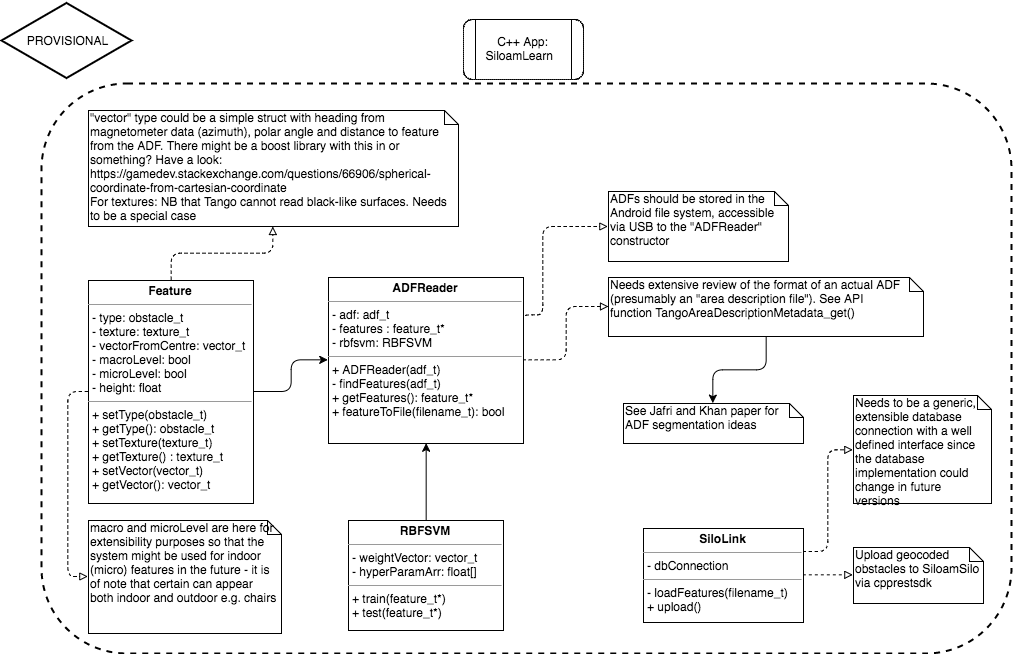
\includegraphics[scale=0.4]{SiloamLearn}
	\caption{SiloamLearn: RGB-D Machine Learning}
	\label{fig:SLearn}
\end{figure}
 
Centred around the ADFReader class, and its associated methods, the first task of SiloamLearn is to automatically detect and extract the ``floor'' plane from the 3D mesh. Also inspired by Fehr et al. \cite{fehr_covariance_2016}, this will be accomplished by first rendering a set of 120 degree field of views from the centre of the 3D mesh and subtracting the floor via the commonly used RANSAC algorithm. The findFeatures method will then segment any objects found in the scene and generate a feature vectors, comprising of position, colour, image intensity, output of the Sobel \cite{gonzalesdigital} operator, depth finally and surface normal data. The RBFSVM object in figure \ref{fig:SLearn} will be trained with a combination of feature vectors generated from a combination of 3D meshes of outdoor macro level objects captured in the wild and models from openly accessible databases including the Trimble 3D Warehouse \cite{trimble_inc._3d_nodate}. Subject to experimental performance in the methods outlined in section \ref{evalDesign}, the features that will be detected will be in the set \{lamp post, bus stop, doorway, steps\}. Figure \ref{fig:scenes} shows example meshes captured with the available RTAB-Map for Android Tango devices set at a capture depth of 2.5 metres (the default for the application, it is possible that optimisations are not ideal beyond this distance). The top area of figure \ref{fig:scenes} (a) shows part of a car which was black in colour, highlighting the difficulty in rendering capturing data for dark objects. Interestingly however, the leftmost extreme of Figure \ref{fig:scenes} (b) shows a globe object on top of a pillar with a partially visible black cross set into white. During capture, the cross was not visible in the UI. The cross is however rendered which suggests negative searching may take place and used to compensate dark areas. Figure \ref{fig:scenes} shows a lamp post on the left and a tree on the right. The tree is mostly rendered correctly but the partial lamp post has an artifact rendered off to around the 11 o'clock direction, highlighting some inaccuracies in depth capture. These limitations might make the use of the open source tool MeshLab \cite{cignoni_meshlab:_2008} necessary, which features an array of automatic and semi-automatic mesh fixing and hole filling tools. This would be particularly useful for situations like those in figure \ref{fig:scenes} (c) where a jagged hole is visible in a portion of the top part of the pillar.

ADFReader will then save the features to a file encoded in JSON format. The representation of each feature will encode the category of the object in the the set \{lamp post, bus stop, doorway, steps\}, its GPS location in relation to the central GPS point where the RGB-D photo sphere was captured, its height and the kerb height closest to the same GPS point. If there is no kerb in the region, the kerb height will be set to -1. This file will then be read by the SiloLink class and a connection will be made to the database system outlined in section \ref{SSilo}, for which the open source Microsoft cpprestsdk \cite{noauthor_cpprestsdk:_2017} will be used.   

\begin{figure}
\centering
    \subfloat[]{
      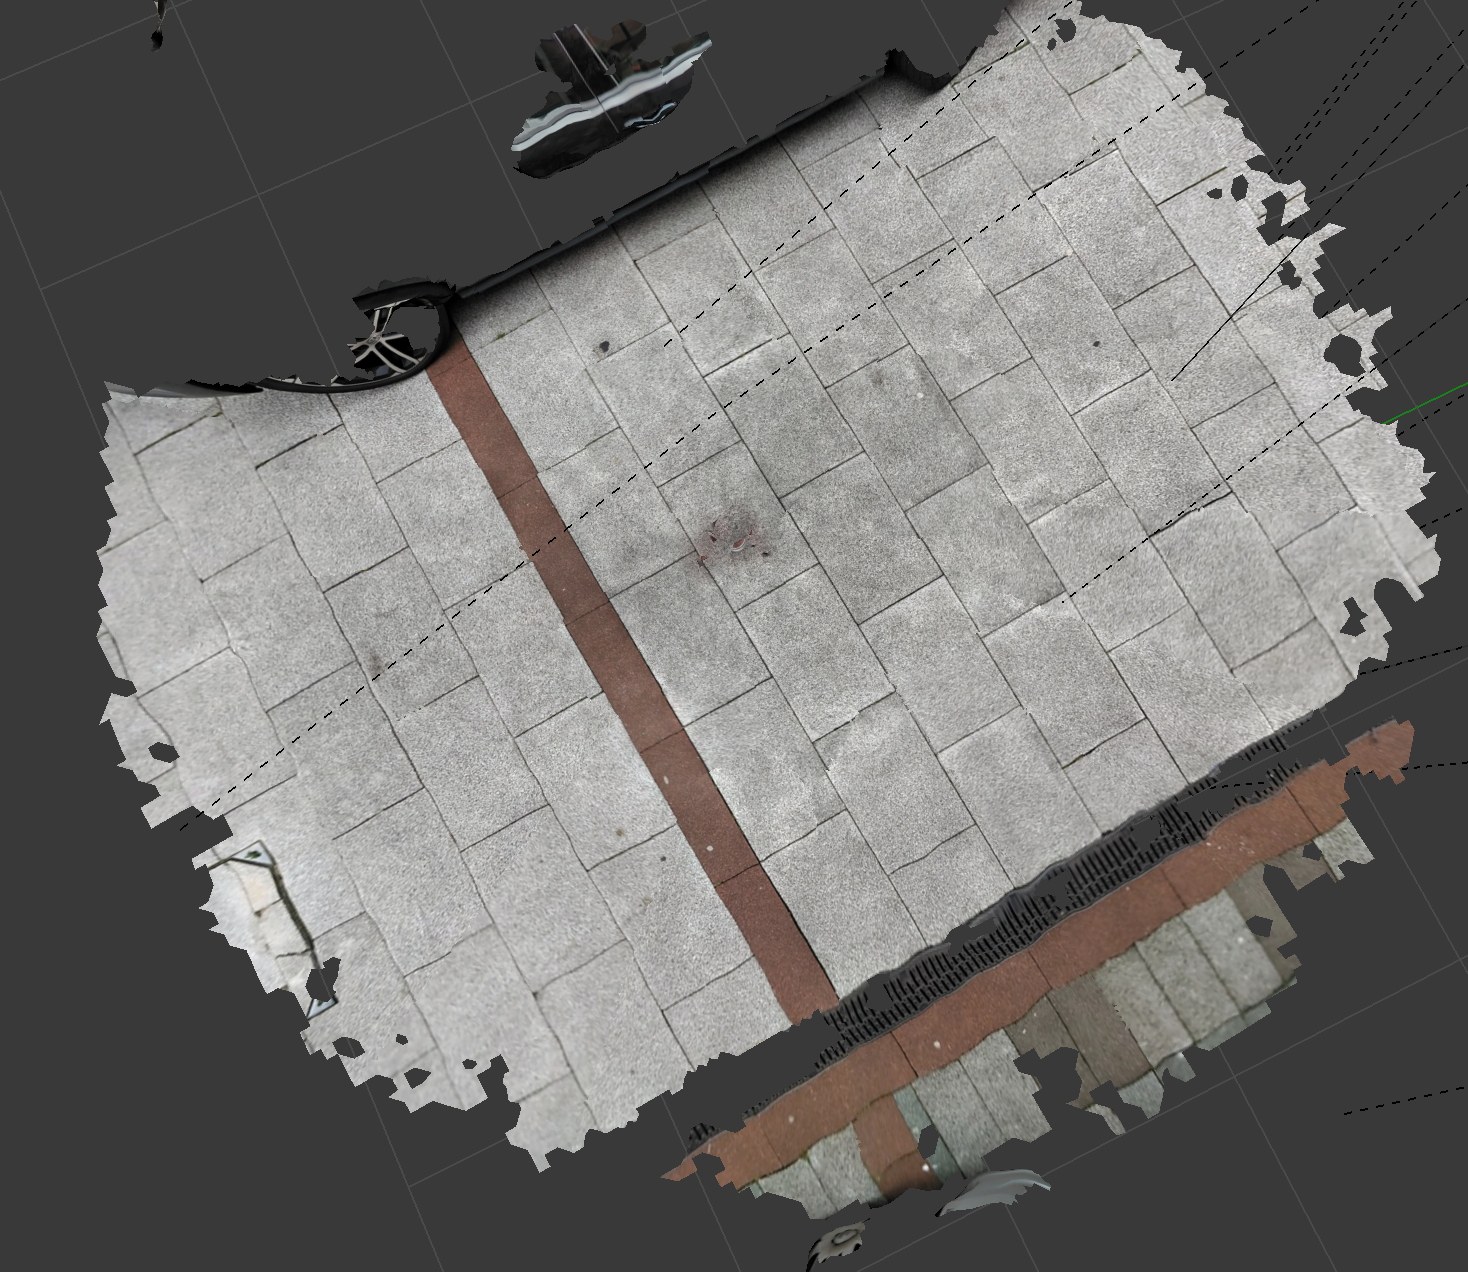
\includegraphics[width=65mm]{sceneFloor}
    }
    \subfloat[]{
      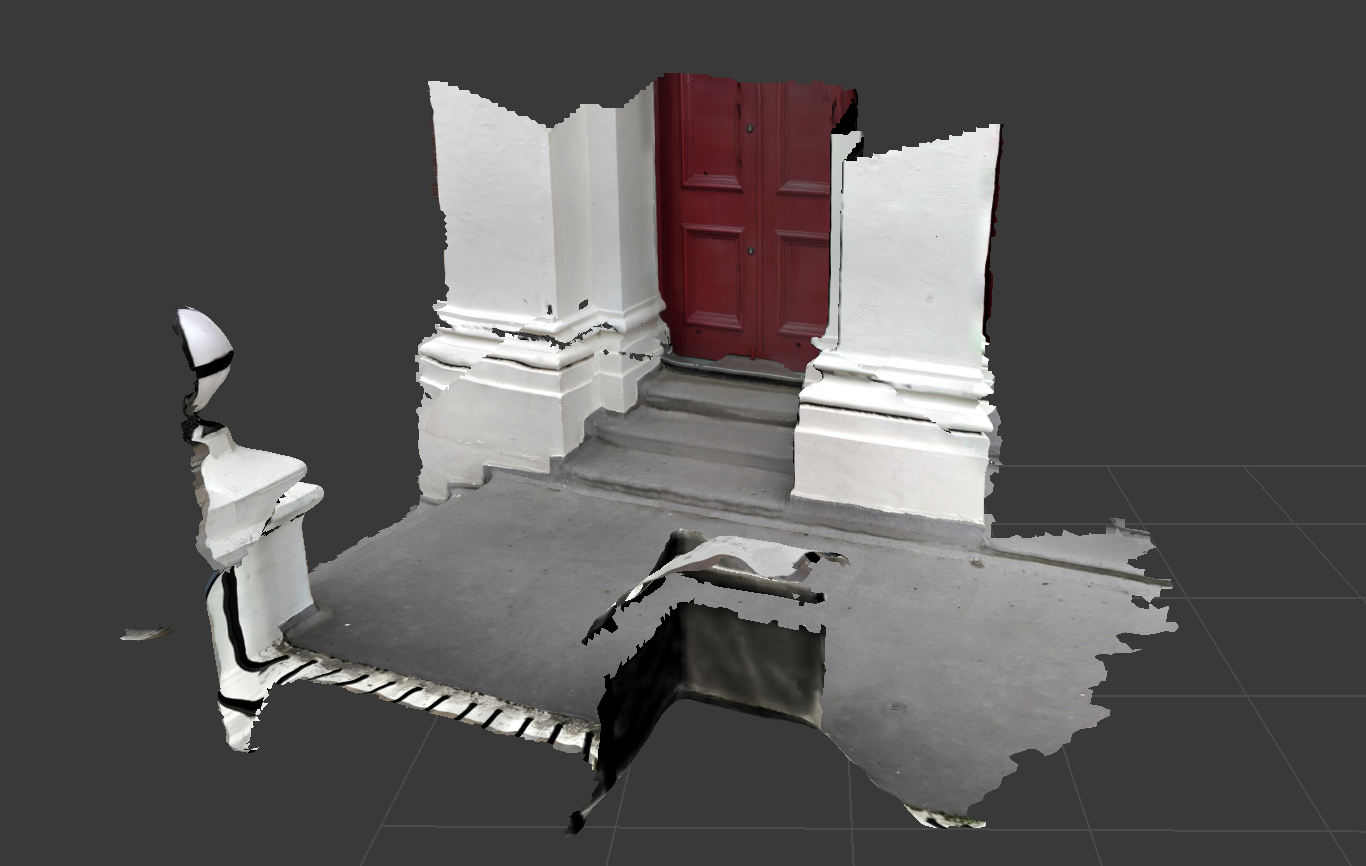
\includegraphics[width=65mm]{sceneDoor}
    }
    \hspace{0mm}
    \subfloat[]{
      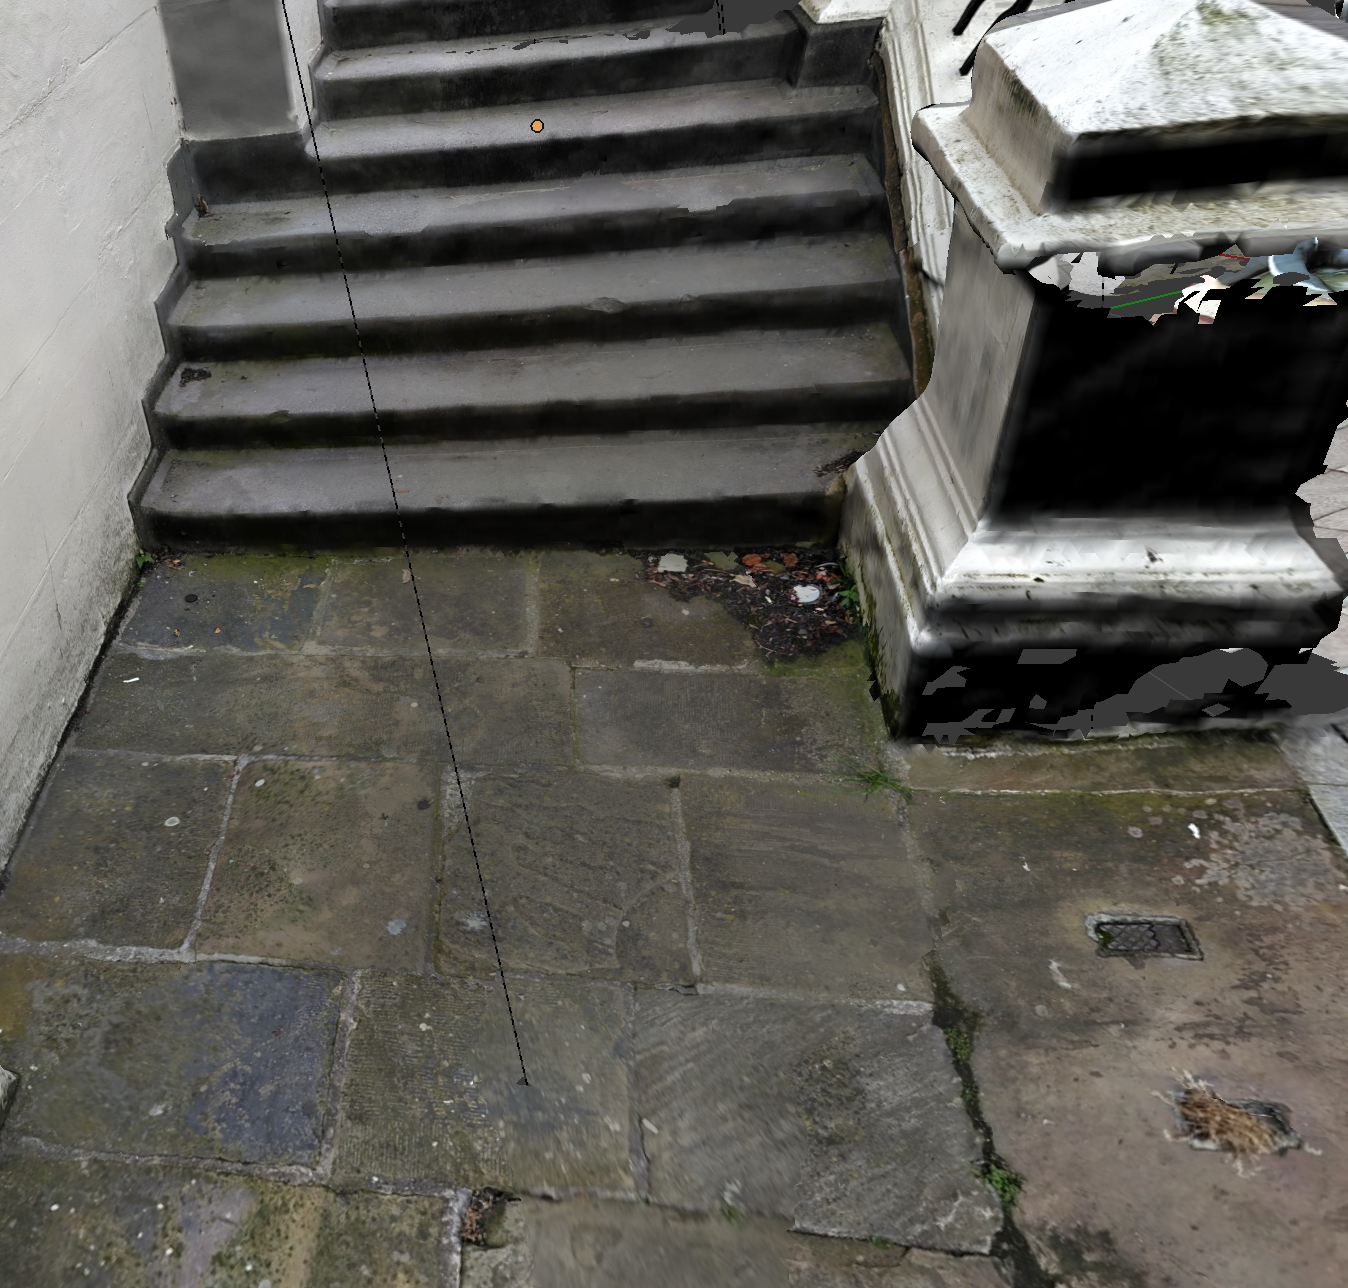
\includegraphics[width=65mm]{sceneSteps}
    }
    \subfloat[]{
      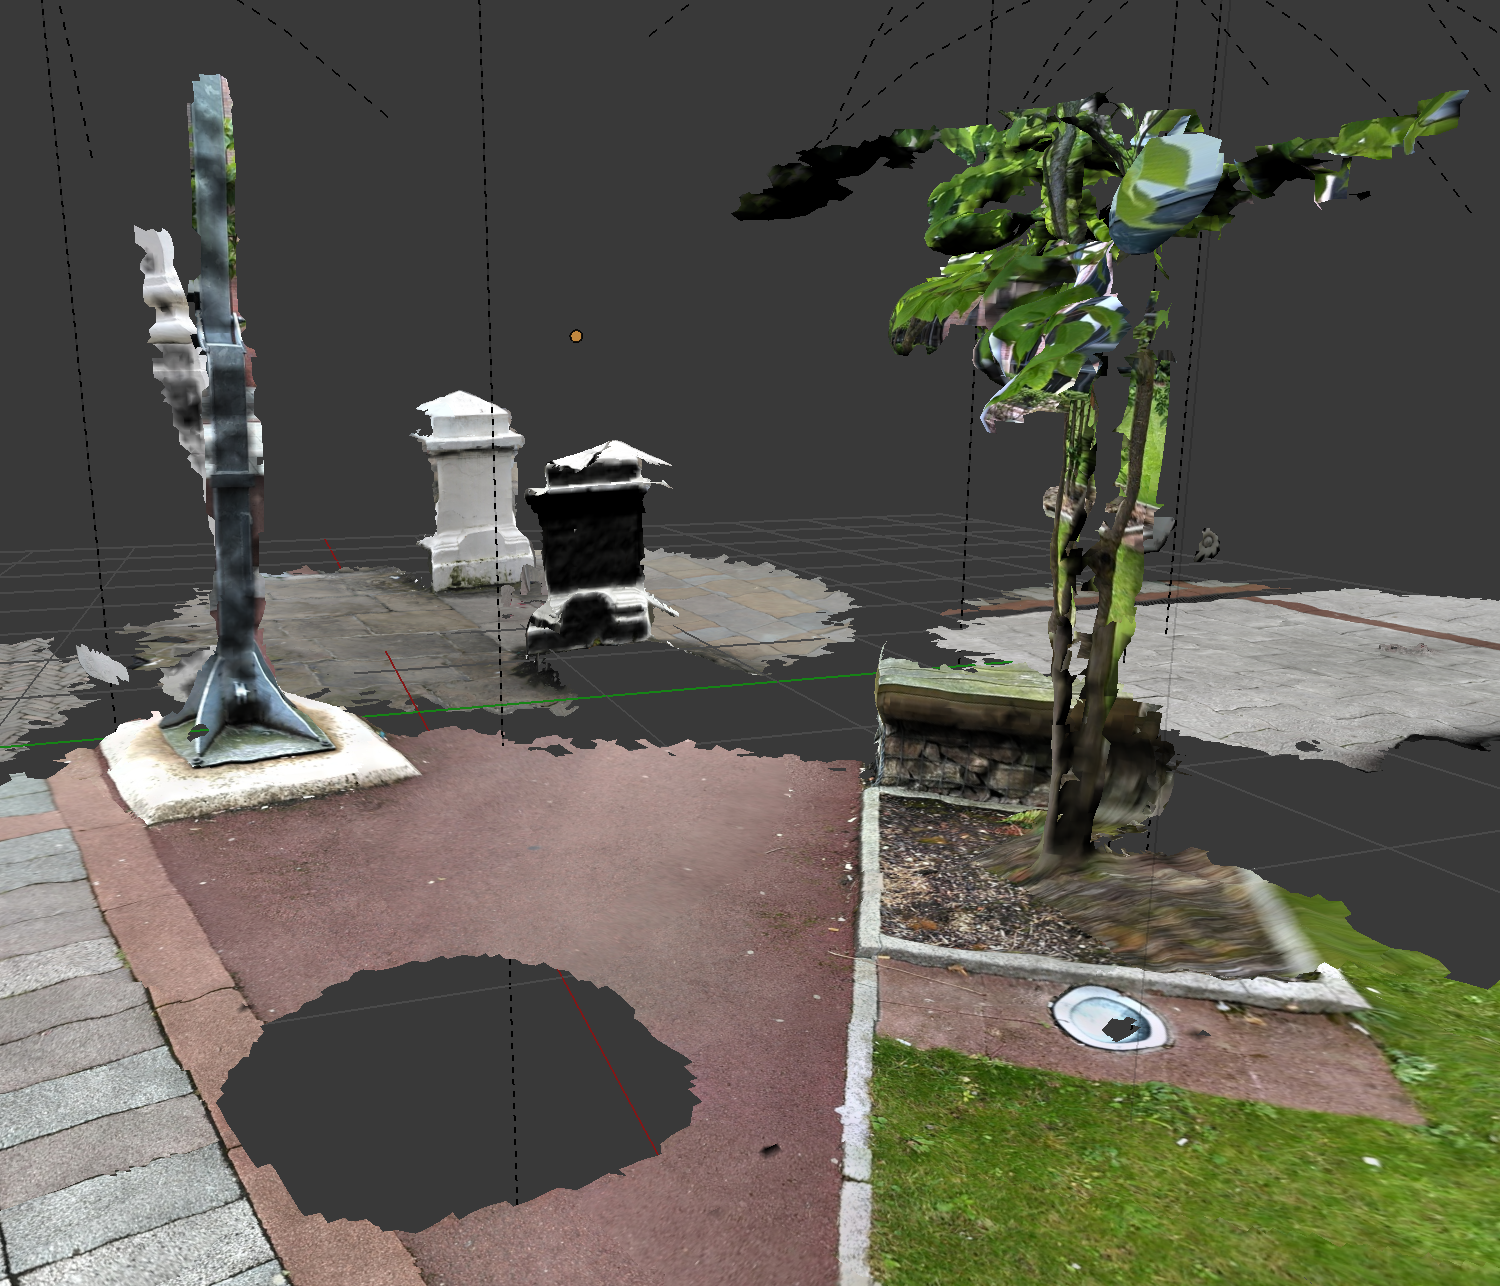
\includegraphics[width=65mm]{sceneLampTree}
    }
    \caption{Examples of 3D meshes captured with RTAB-Map and rendered with Blender. Visible dotted black lines are Blender light ray paths, not captured textures (a) simple floor (b) steps and doorway (c) steps and pillar (d) streetlamp and tree}
    \label{fig:scenes}
\end{figure}  

\subsection{SiloamSilo}\label{SSilo}

While a schema design is currently in development, the datastore of the system (hinted at in section \ref{secSLearn}), SiloamSilo, will make use of the Apache CouchDB database \cite{noauthor_couchdb:_2017} with the geocouch extension to allow spatial queries to the database \cite{noauthor_geocouch:_2017}. Figure \ref{fig:SSilo} shows a brief overview of the system as well as its interaction with SiloamRoute, the routing subsystem developed by my colleague.  

\begin{figure}[h]
\centering
	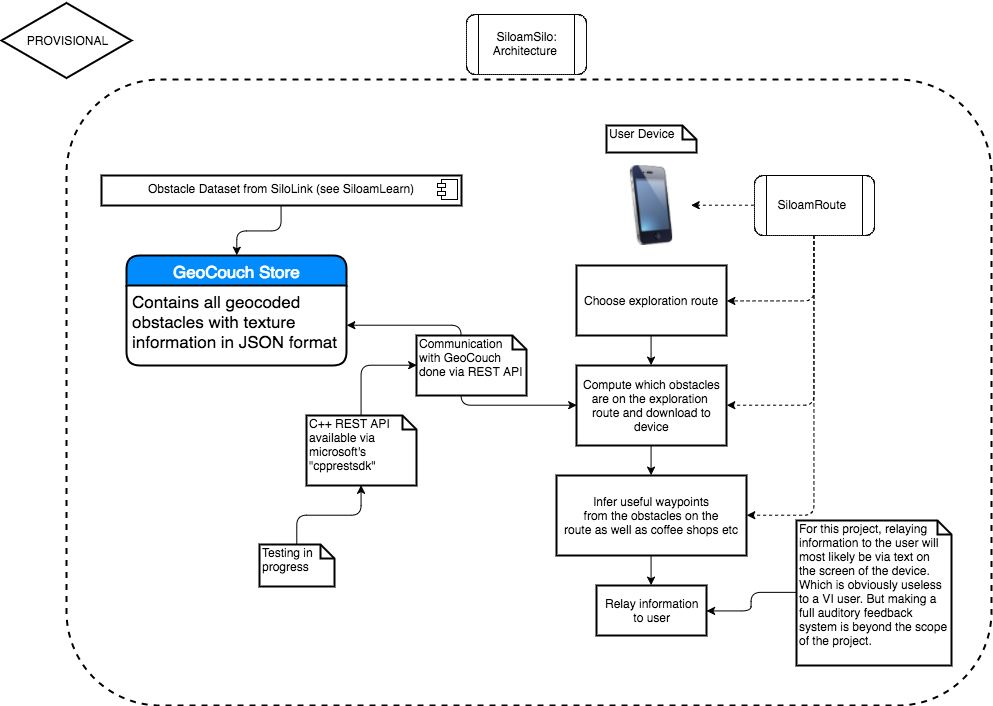
\includegraphics[scale=0.4]{SiloamSilo}
	\caption{SiloamSilo: Data Organisation and brief overview of SiloamRoute}
	\label{fig:SSilo}
\end{figure}

\section{Evaluation Design}\label{evalDesign}

The area to be mapped is the UoL campus. Therefore, it makes sense to train the SiloamLearn component on certain areas and then test on other, unseen portions of it. These areas are visualised in figure \ref{fig:testTrainMap}. Areas in red will be captured for SVM training purposes while those highlighted in blue are considered for testing. It is possible that blue regions may be encapsulated within the training regions as development progresses due to higher concentrations of macro level street level features. 

For an evaluation run, a simple approach whereby feedback from the testing device will be noted and compared to the actual surroundings at any given location. From these, precision and recall characteristics of the system can be produced.

As a separate stage in evaluation, the route heading approximately north between the intersection between Myrtle Street and University square (the uncoloured region that splits red and blue training and testing areas) will be a ground truth route. That is, an entire 3D map of this route will be scanned and annotated by hand. This route will remain completely unseen in both testing and training phases and will be used as another evaluation metric. 

\begin{figure}[h]
\centering
	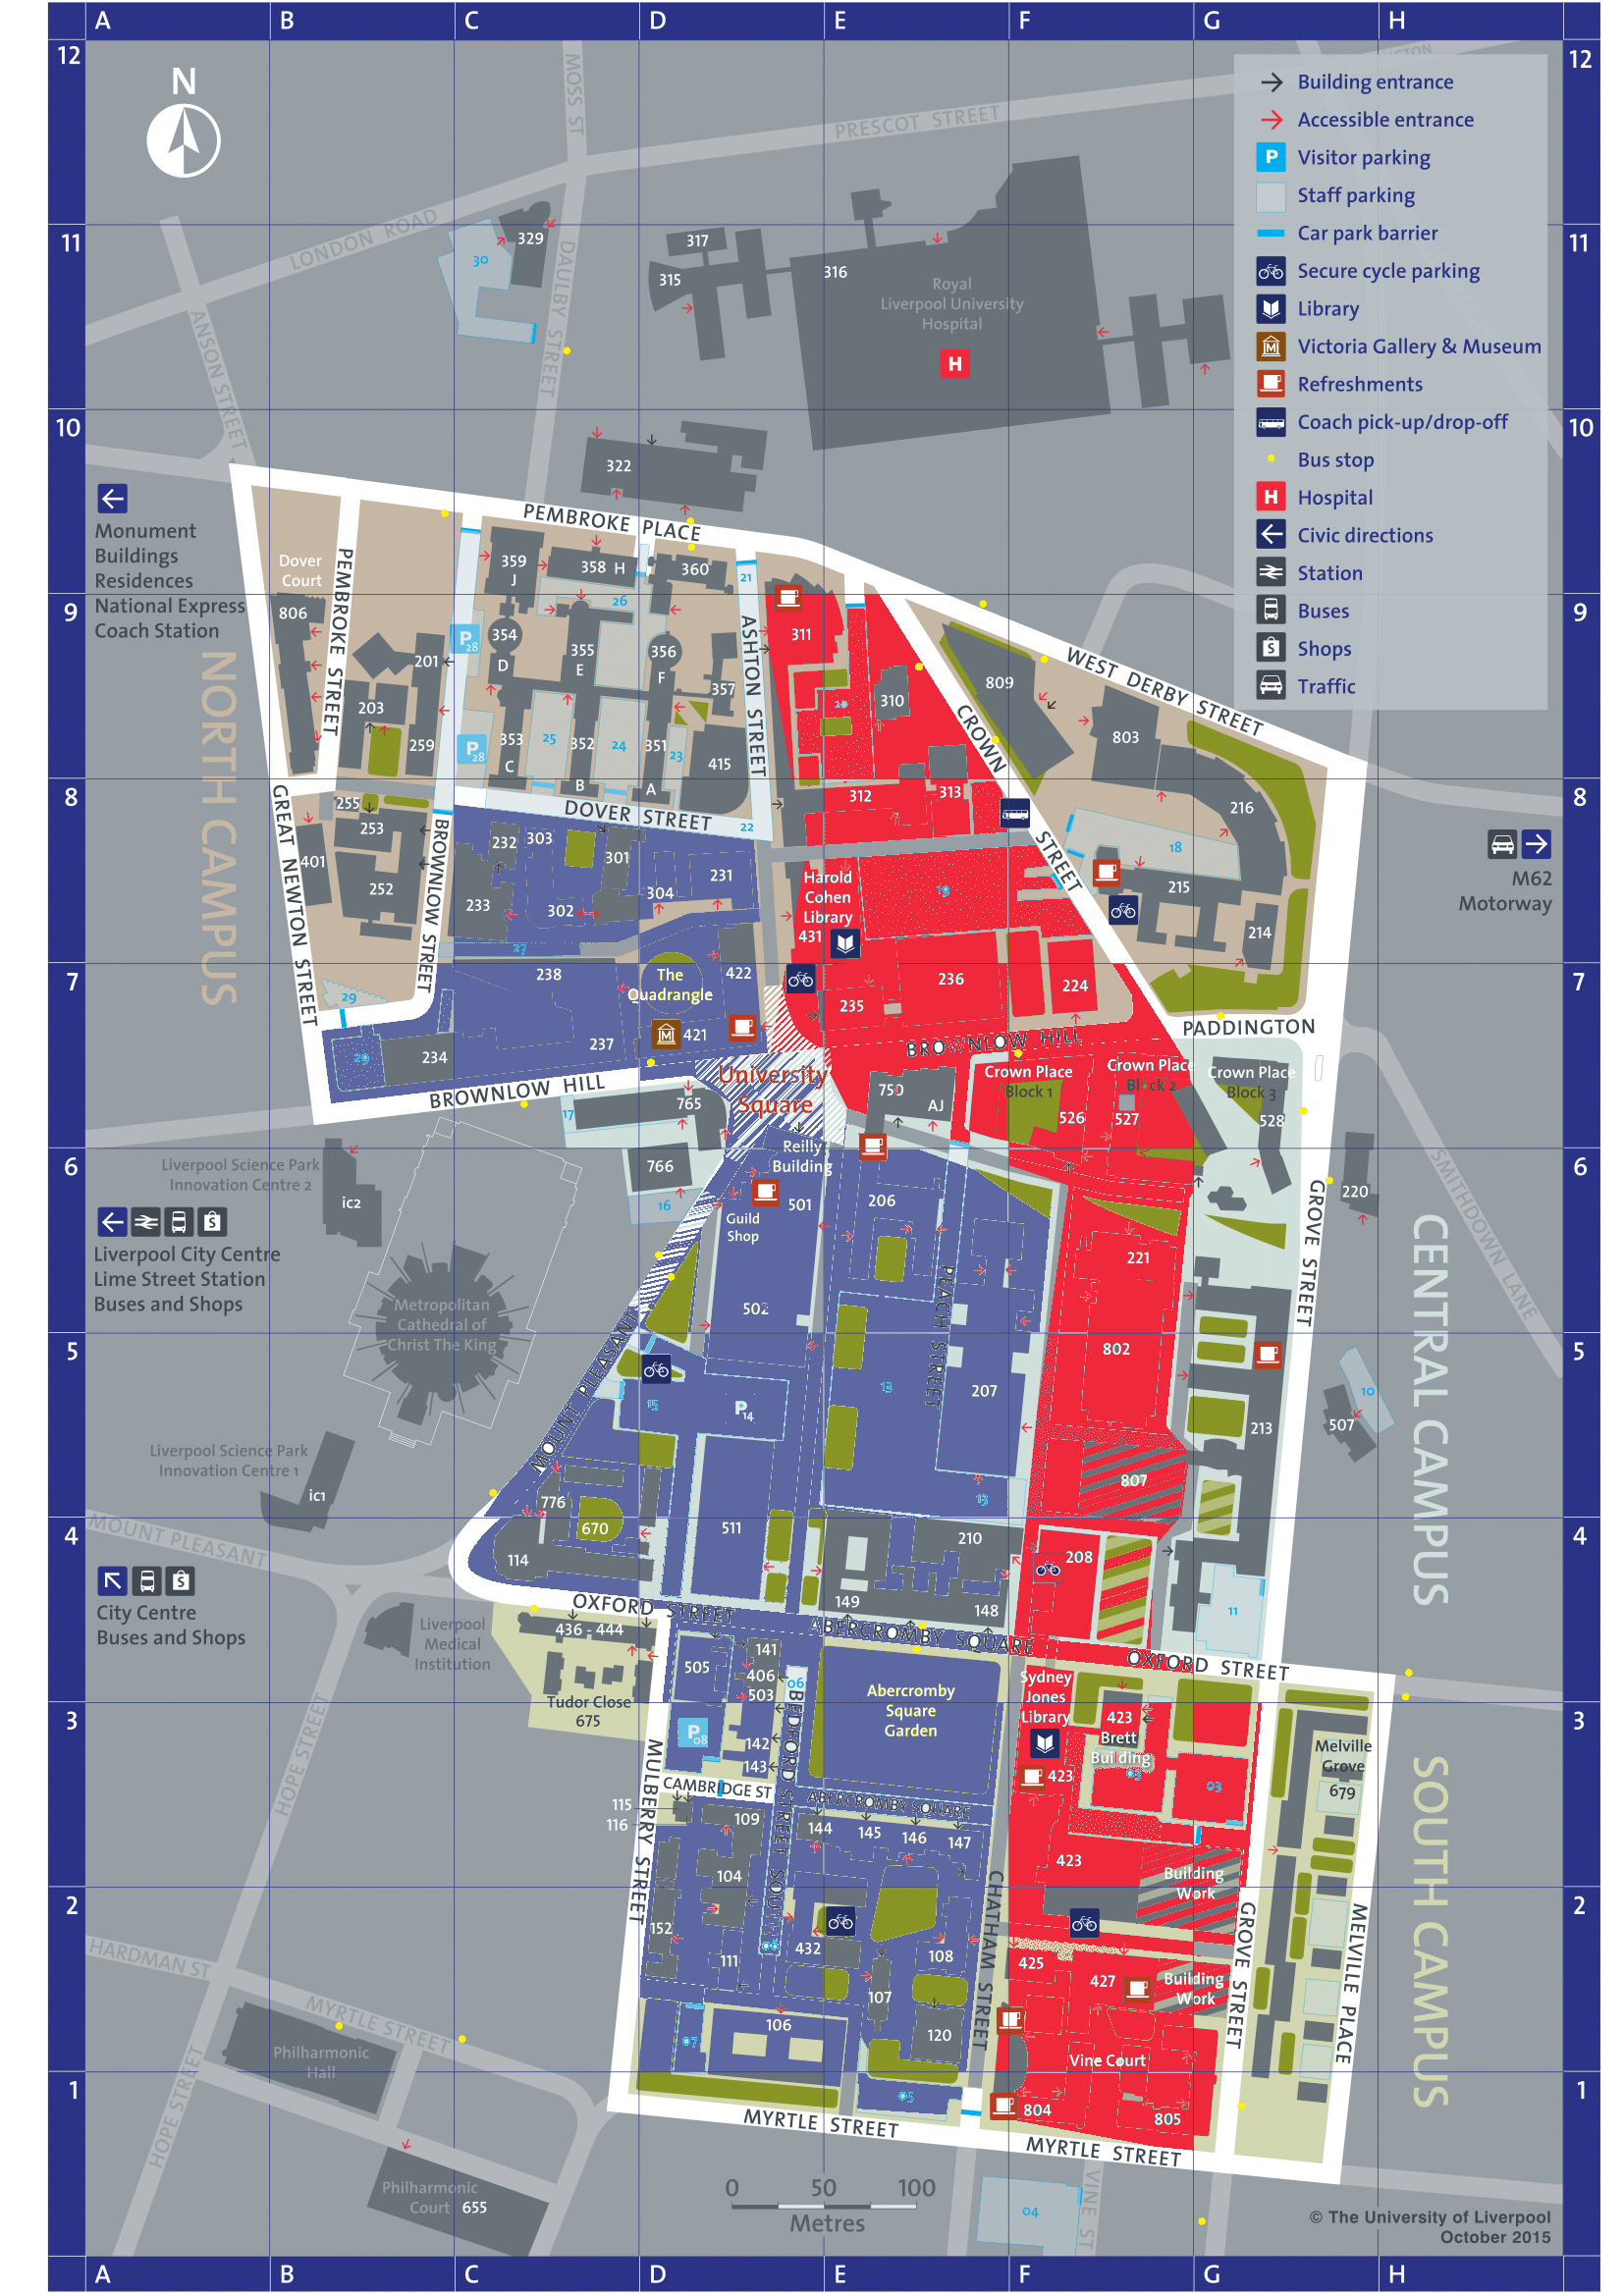
\includegraphics[scale=0.2]{trainTestRegions}
	\caption{Train and Test Regions of Siloam. Red regions are used for training, blue regions are considered for testing}
	\label{fig:testTrainMap}
\end{figure}

%%%%  DATA REQUIRED

\chapter{Data}\label{chap:data}

\section{Data Collection}

Since this project aims to form a standard for data collection to improve quality of life for BoVI users, much of the data collected will be the first of its sort. Data collection schemes and use of external freely available data like 3D models from the Trimble warehouse \cite{trimble_inc._3d_nodate} are covered in detail in sections \ref{secSSee} and \ref{secSLearn}.

\section{Ethical Use of Data}

It is a non trivial task to predict the level of the activity of pedestrians and cars in public areas. Given this, at many points during outdoor RGB-D data capture texture information of faces or vehicle number plates may be accidentally recorded. As part of SiloamSee and taking inspiration from Street View, an interactive effort to blur out these features in order to anonymise data is required. This functionality will be included within the system detailed in section \ref{secSSee}. 

%%%% RISK ASSESSMENT

\chapter{Risk Assessment}\label{chap:risk}

\begin{longtable}{ | p{3cm} | p{2cm} | p{2.2cm} | p{3cm} | p{3cm} | }
\hline
 Risk & Likelihood &  Consequence & Risk Management Approach & Risk Symptoms \\ 
 \hline
 \hline
 Falling seriously ill  & Low(1) & High(4) & Go to the gym regularly, eat well, get plenty of rest & General sense of malaise, aches and/or pains, any symptoms which require a GP visit/sudden accident resulting in serious injury \\ 
 \hline
 Catastrophic data loss on personal and/or university computers due to personal error or otherwise & Med(2) & Very High(5) & Back up data and development code to external HDD regularly and github & Return to development machine to find the files required no longer exist/have been rolled back to a much earlier version with no method of recovery \\ 
 \hline
 The covariance descriptor method combined with the RBF SVM does not result in usable performance figures & Med(2) & High(4) &  During development of SiloamLearn, always keep in mind other classification descriptors like those detailed in table 1 of Fehr et al. \cite{fehr_covariance_2016} & Classification accuracy is consistently below 80\% \\ 
 \hline
 Development of SiloamEyes is not completed within time constraints. Since this must be completed before other components of the project are completed, this is a serious event. & Med(3) & Med(3) & SiloamLearn is the principle aim of the project, so a simpler, file based rather than database based, approach to SiloamSilo could be implemented. The plan in chapter \ref{chap:plan} also gives ample time for experimentation. Given the nature of this project experimentation will be on ongoing process throughout all parts of the project so a certain amount of slack time can be taken from this & SiloamEyes is not completed by 09/07/2017 \\ 
 \hline
\end{longtable}

%%%% PLAN

\chapter{Plan}\label{chap:plan}

``Timeboxing'' is another concept borrowed from the DSDM \cite{bittner2002use}. It is used to gauge if development is on time concerning the desired quality is what is produced on a given project. Project elements that are at different levels of priority have been identified by the \textbf{M}o\textbf{SC}o\textbf{W} principle in chapter \ref{chap:design}. A gantt chart showing the timeboxing plan is shown in figure \ref{fig:gantt} which includes the various milestones of the project. Various overlaps are shown in the timeboxes, including between the SiloamLearn and SiloamSilo components. These overlaps exist to maximise use of time. 

\begin{figure}[H]
\centering
	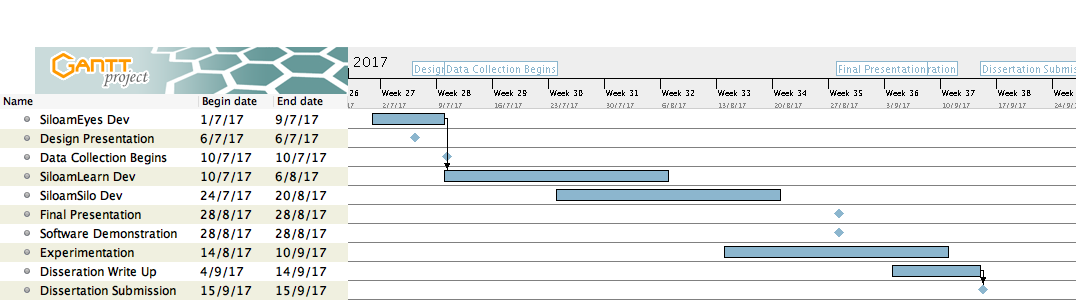
\includegraphics[scale=0.4]{provPlan}
	\caption{Proposed timeboxing plan}
	\label{fig:gantt}
\end{figure}

\noindent \textbf{NB}: an internal dissertation submission date is applied due to future employment constraints imposed on the author.

%%%%   REFERENCES

%%%%  Section for references, using the \bibitem directive to 
%%%%  specify labels used to cite sources in the document.  

\bibliographystyle{IEEEtran}
%\bibliographystyle{plain}
\bibliography{References}

\end{document}
